\scanpage{94}
\margin{\figure{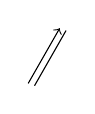
\begin{tikzpicture}[x=1cm,y=1cm]\draw[->](0,0)--(.4,.7);\draw(.08,-.03)--(.48,.67);\end{tikzpicture}} N.B. le critère implique \unsure{la condition|le critère} d'amplitude de A. Weil ....}

\uline{Th de Mumford-Nakai}\qquad $X$ schéma projectif sur corps $k$,
$L$ faisceau inv. sur $X$. Conditions équivalentes :

a) $L$ ample

b) Pour $\forall$ \deleted{sous-préschéma fermé intègre $Z$ de $X$}\inserted{faisceau cohérent $F$ sur $X$} \deleted{\unsure{de dim}} $\dim\operatorname{supp}F\geq1$, on a
\[
\chi(F\otimes L^{\otimes n})\longrightarrow+\infty\qquad\text{si }n\longrightarrow+\infty.
\]

b') Comme b), avec $F$ de la forme $\mathcal O_Z$, $Z$ un sous-préschéma intègre de $X$ de $\dim\geq1$.
\margin{on peut se borner à \uline{supposer}}

\unsure{b''}) Pour $\forall$ sous-préschéma intègre $Z$ de $X$, tels que $\dim Z=1$ (resp. $\dim Z\geq2$), il existe un entier $n=n_Z>0$ tel que
\[
\chi(L^{\otimes n}\otimes\mathcal O_Z)\geq2
\]
(resp. $\chi(L^{\otimes n}\otimes\mathcal O_Z)\geq1$).

c) Comme b), \uline{en remplaçant $\chi$ par} \deleted{\unsure{H}} $\dim H^0$

c') Comme b')

c'') Pour $\forall$ sous-préschéma intègre $Z$ de $X$ \inserted{$\boxed{\text{tels que }\dim Z=1\ (\dim Z\geq\unsure{1|2})}$} existe un entier $n=n_Z>0$ tel que
\[
\dim H^0(Z,L^{\otimes n}\otimes\mathcal O_Z)\geq2
\]
(resp. $\geq1$).

\margin{\uline{Critère numérique} ($X$ \unsure{irred} de dim $d$)
\[
\left\{\begin{array}{l}
D.C>0\quad\text{si }C\text{ courbe \unsure{irred}}\ \deleted{\unsure{de X}}\ >0\\
D^d>0
\end{array}\right.
\]
(\unsure{intersections} \unsure{calculées|calculés} dans $CK(X)$!)}

\deleted{d) Il existe un entier $\unsure{n|\nu}>0$ tel que $L^{\otimes\unsure{n|\nu}}$ admette une section\inserted{${}\neq0$}; et pour tout sous-préschéma intègre $Z$ de $X$, \deleted{il existe un}\inserted{\uline{de dim 1}}, il existe un entier $n>0$ tel que
\[
\dim H^0(Z,\unsure{L^{\otimes n}_{\otimes\mathcal O_Z}|L^{\otimes n}\otimes\mathcal O_Z})\geq2.
\]}

\deleted{d') \deleted{Pour} Il existe un entier $n>0$ tel que $L^{\otimes n}$ admette une section\inserted{${}\neq0$}, et pour $\forall$ sous-préschéma intègre $Z$ de $X$, de dim 1, on a $\deg(\unsure{L\otimes\mathcal O_Z|L\vert_Z})>0$.}

\margin{93\quad$\unsure{\xi}\,1$}
